\documentclass[a4paper]{article}

%% Language and font encodings
\usepackage[english]{babel}
\usepackage[utf8x]{inputenc}
\usepackage[T1]{fontenc}

%% Sets page size and margins
\usepackage[a4paper,top=3cm,bottom=2cm,left=3cm,right=3cm,marginparwidth=1.75cm]{geometry}

%% Useful packages
\usepackage{amsmath}
\usepackage{graphicx}
\usepackage[colorinlistoftodos]{todonotes}
\usepackage[colorlinks=true, allcolors=blue]{hyperref}
\usepackage{braket}
\title{QM Problems}
\author{Anoop Chandran -- Lorenzo Fant}

\begin{document}
\maketitle


\section{A. Solid Argon With LJ Potential}
NOTE: The code and related documents are available in the GitHub repo created for this project \\
https://github.com/lorenzofant/QMprob2
\subsection{Lattice Parameters}
From the general expression of the Lennard-Jones potential
\begin{equation}
V(r) = 4\epsilon\left(\left(\frac{\sigma}{r}\right)^12-\left(\frac{\sigma}{r}\right)^6\right)
\end{equation}
We can easily find the minimum finding the zero of the first derivative.
\begin{equation}
r_0 = 2^{\frac{1}{6}}\sigma
\end{equation}
and, substituting it into the potential expression we find
\begin{equation}
V(r_0) = -\epsilon
\end{equation}
From these two expressions we can deduce $\sigma = \frac{3.758}{2^{\frac{1}{6}}}$\AA and $\epsilon = 99.55 cm^{-1}$
\subsection{Crystal Structures}
Knowing the expression for the Lennard-Jones potential we can derive an approximate value of the energy of different lattice structures by numerically summing the potential energy contributions of the neighbours.
\begin{figure}[h]
    \centering
    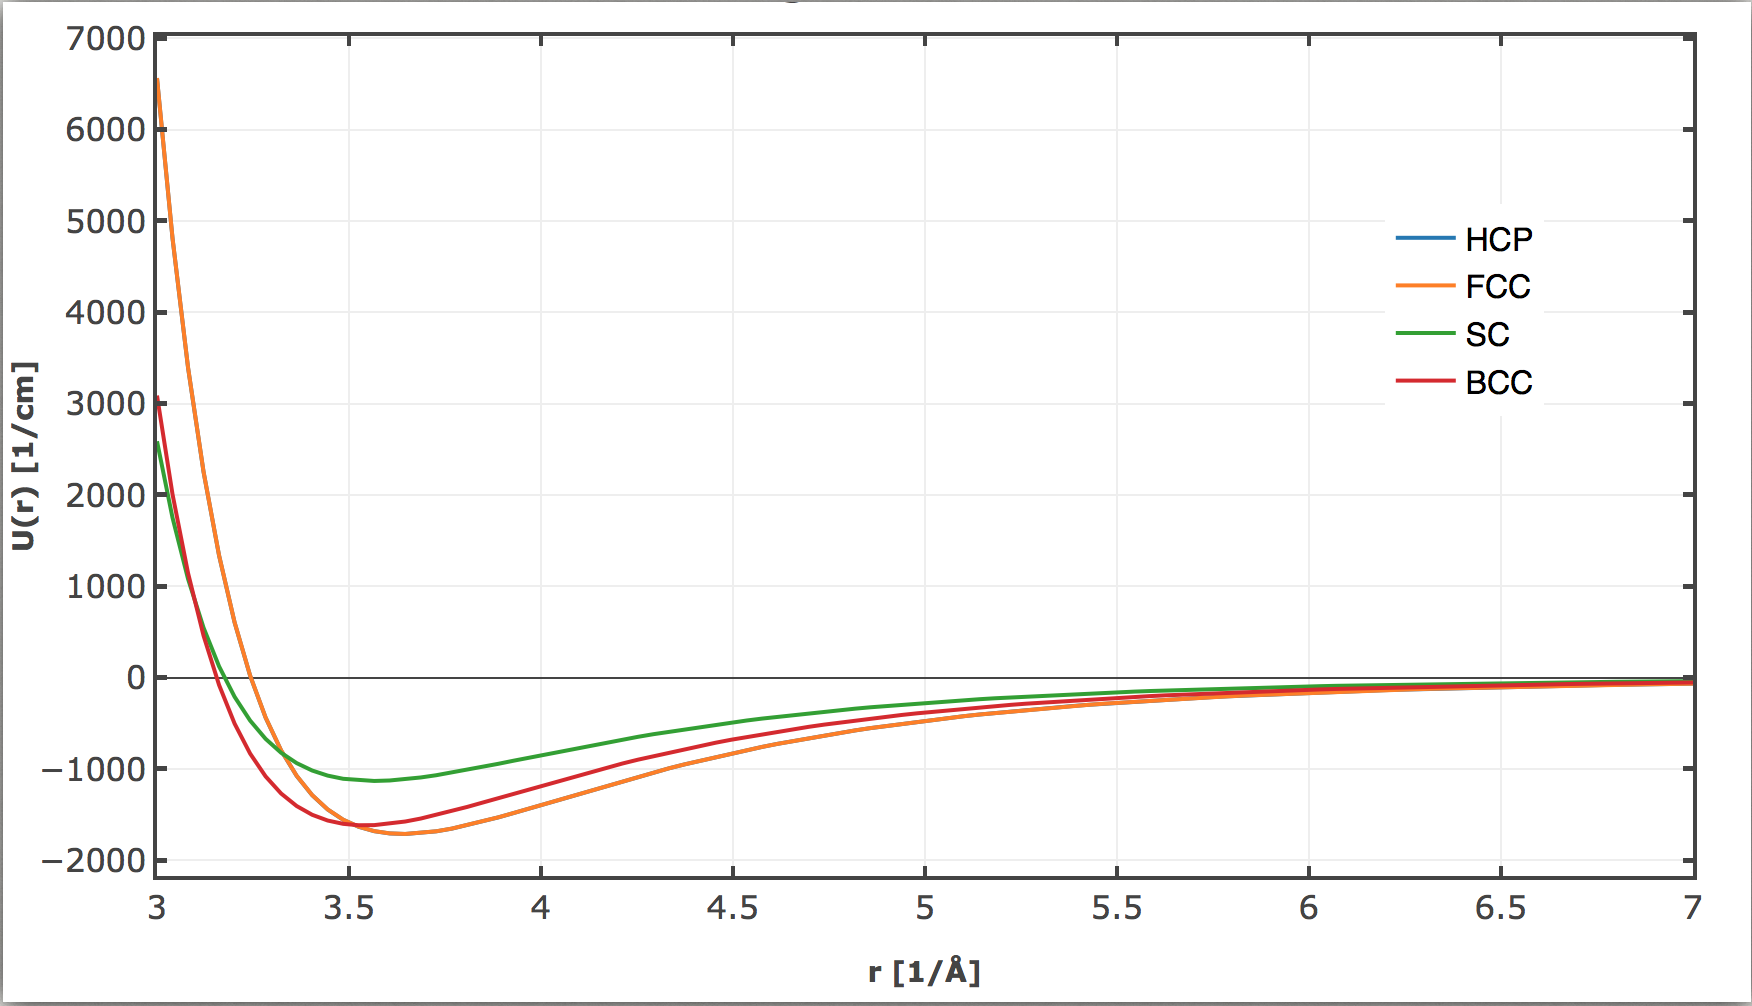
\includegraphics[width=12cm]{lj.png}
    \caption{\it \label{en(spacing)}Energy of the atoms in the lattice as a function of the lattice spacing for four possible lattices: Simple Cubic (Blue), Face Centered (Green), Body Centered (Red), hexagonal Centered (Light blue)}
\end{figure}
    
Doing so for the $14^3$ closest neighbours, we found the following values for the required structures
\begin{eqnarray*}
&spacing&energy\\
sc&1.066\sigma&-11.36\epsilon\\
bcc&1.069\sigma&-16.45\epsilon\\
fcc&1.090\sigma&-17.2160\epsilon\\
hcp&1.090\sigma&-17.2192\epsilon
\end{eqnarray*}
We thus found that the energetically favourable configuration is the $hcp$ one by a factor of $0.01\%$ with respect to the $fcc$.
This is in agreement with results found in the literature ref{crystal}. 
In the same reference it is also pointed out that despite $hcp$ configuration being lower in energy, the one that more easily appears in nature is the $fcc$ one.
We here try to justify such a result without considering, as done in \ref{crystal}, impurities.\\
We tried instead to consider the behaviour of the energy in the minimum when some random noise is present in the lattice, displacing the positions of the atoms.
We looked at the behaviour of the energy as a function of the amplitude of the noise averaging over $10^4$ different realisations of the system with a Gaussian random displacement of amplitude $d$.

\begin{figure}[ht]
    \centering
    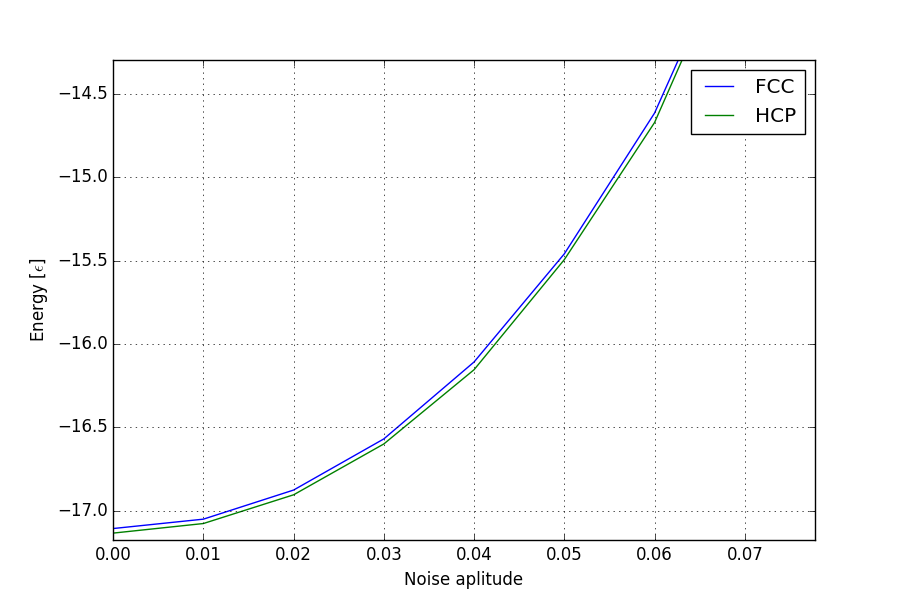
\includegraphics[width=12cm]{energy_noise.png}
    \caption{\it \label{noise}Energy of the minima obtained above for FCC and HCP lattices as a function of the amplitude of a random noise displacing the atoms positions}
\end{figure}

We can see that there is no crossing between the two energies and thus it the fact that the FCC structure is preferred in nature cannot be explained in this way.
The next step would be to simulate different potential models such as Barker-Fisher-Watts (BFW) potential\cite{bfw} and Aziz-Chen (Hartree-Fock, HFD-C) potentials\cite{hfd}
 to see whether they find any results different than the one obtained using L-J potential. Even though BFW finds a new minima for the energy the HPC structure still have the minimum among
 the crystal structures. An improved version of this BFW known as Barker-Bobetic-Maitland-Smith (BBMS) potential\cite{bbms} which best describes Argon behaviour can be found in the literature. as shown in the figure \ref{diff-pot}
 \begin{figure}[h]\label{diff-pot}
    \centering
    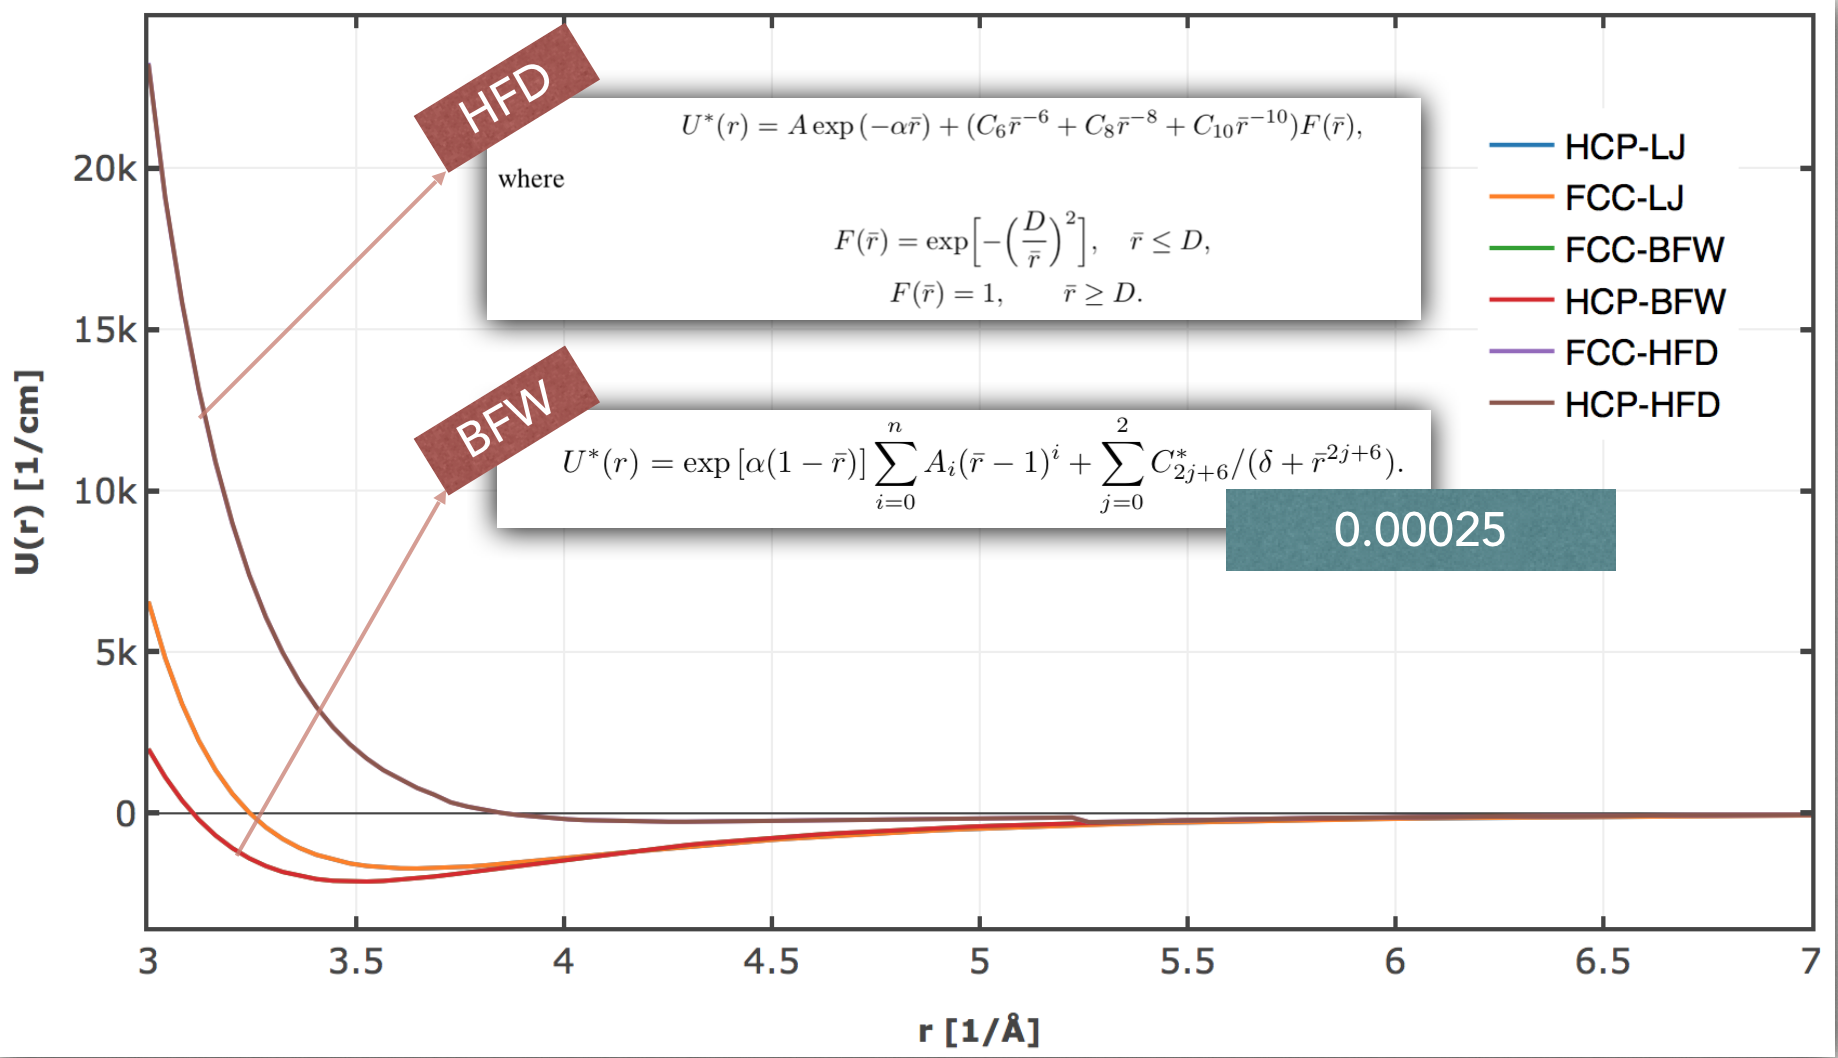
\includegraphics[width=12cm]{diff_pot.png}
    \caption{\it \label{diff-pot}Energy of the atoms in the lattice as a function of the lattice spacing for four possible lattices: Face Centered , hexagonal Centered for BFW and HFD potentials }
\end{figure}
\subsection{Spectrum of the HCP}

In the case of the HCP configuration we find a structure where we have two atoms per unit cell.
The cell can be easily identified through the three vectors of coordinates\\
\begin{minipage}{0.3\textwidth}
\centering
\begin{equation*}
R_1 = a
\begin{bmatrix}
	1 \\
    0 \\
    0 \\
    
\end{bmatrix}
\end{equation*}

\end{minipage}
\begin{minipage}{0.3\textwidth}
\centering
\begin{equation*}
R_2 = a
\begin{bmatrix}
    \frac{1}{2} \\
    \frac{\sqrt{3}}{2}  \\
    0 \\
\end{bmatrix}
\end{equation*}
\end{minipage}
\begin{minipage}{0.3\textwidth}
\centering
\begin{equation*}
R_3 = a
\begin{bmatrix}
    0 \\
    0 \\
    2\sqrt{\frac{2}{3}} \\
\end{bmatrix}
\end{equation*}
\end{minipage}



and that of the corresponding reciprocal lattice vectors can be constructed from those above and their coordinates are \\
\begin{minipage}{0.3\textwidth}
    \centering
    \begin{equation*}
    G_1 = \frac{2\pi}{a}
    \begin{bmatrix}
        0 \\
        0 \\
        \sqrt{\frac{3}{2}}\pi \\
        
    \end{bmatrix}
    \end{equation*}
    
    \end{minipage}
    \begin{minipage}{0.3\textwidth}
    \centering
    \begin{equation*}
    G_2 = \frac{2\pi}{a}
    \begin{bmatrix}
        0 \\
        \frac{2}{\sqrt{3}}  \\
        0 \\
    \end{bmatrix}
    \end{equation*}
    \end{minipage}
    \begin{minipage}{0.3\textwidth}
    \centering
    \begin{equation*}
    G_3 = \frac{2\pi}{a}
    \begin{bmatrix}
        1 \\
        -\frac{1}{\sqrt{3}}  \\
        0 \\
    \end{bmatrix}
    \end{equation*}
    \end{minipage}

    While the second atom in the cell is placed in
    \begin{minipage}{0.3\textwidth}
        \centering
        \begin{equation*}
        R_1 = a
        \begin{bmatrix}
            n_1 + \frac{n_2 + 1}{2} \\
            \frac{\sqrt{3}(n_2 + \frac{1}{3})}{2} \\
            (2n_3 + 1)\sqrt{\frac{2}{3}} \\
            
        \end{bmatrix}
        \end{equation*}
        
        \end{minipage}
        
    To evaluate the spectrum of the phonon dispersion one can evaluate, in the harmonic approximation, the equation 
    \begin{equation}
        \omega^2 u_{i,\alpha, g} = \sum_{m,\beta} \frac{1}{M}\frac{\partial^2 V(r)}{\partial r_{i,\alpha, g}\partial r_{m,\beta,f}}e^{i\underline{q}\underline{r}_{im}}u_{m,\beta, f}
    \end{equation}
    where the approximation on the solution $s_{i,\alpha}=e^{i(\underline{q}\underline{r}_i - \omega)}u_{\alpha}$ was applied assuming the harmonic nature of the system.
    The indices $\alpha,\beta$ can assume values between $x,y,z$, the indices $i,m$ along the cells in the lattice and $g,f$ along the atoms inside the unit cell.
    We can now define 
    \begin{equation}
        \Phi_{\alpha\beta}^{imgf}(r):=\frac{\partial^2 V(r)}{\partial r_{i,\alpha,g}\partial r_{m,\beta,f}}
    \end{equation}
    where the expression for the second derivative of the potential reads
    \begin{equation*}
        \frac{\partial^2 V(r)}{\partial r_{i,\alpha,g}\partial r_{m,\beta,f}} = \sum_{jh}\left[\frac{\partial^2 v(r_{ij})}{\partial r_{ij}^2}\frac{(r_{ij})_{\alpha}(r_{ij})_{\beta}}{r_{ij}^2} + \frac{\partial v(r_{ij})}{\partial r_{ij}}\left(\frac{\delta_{\alpha\beta}}{r_ij}-\frac{(r_{ij})_{\alpha}(r_{ij})_{\beta}}{r_{ij}^3}\right)\right](\delta_{gf}\delta_{im}-\delta_{fh}\delta_{jm})
    \end{equation*}
    and from here the dynamical matrix
    \begin{equation}
        D_{\alpha\beta} = \frac{1}{M}\sum_j\left[\frac{\partial^2 v(r_{ij})}{\partial r_{ij}^2}\frac{(r_{ij})_{\alpha}(r_{ij})_{\beta}}{r_{ij}^2} + \frac{\partial v(r_{ij})}{\partial r_{ij}}\left(\frac{\delta_{\alpha\beta}}{r_ij}-\frac{(r_{ij})_{\alpha}(r_{ij})_{\beta}}{r_{ij}^3}\right)\right]\left(2\delta_{gf}-e^{i\underline{q}\underline{r}_{ij}}\right)
    \end{equation}
    The diagonalization of the former thus brings to the dispersion relation of the phonons. The calculated phonon dispersion is given in the figure \ref{phonon-hcp}
    \begin{figure}[h]
        \centering
        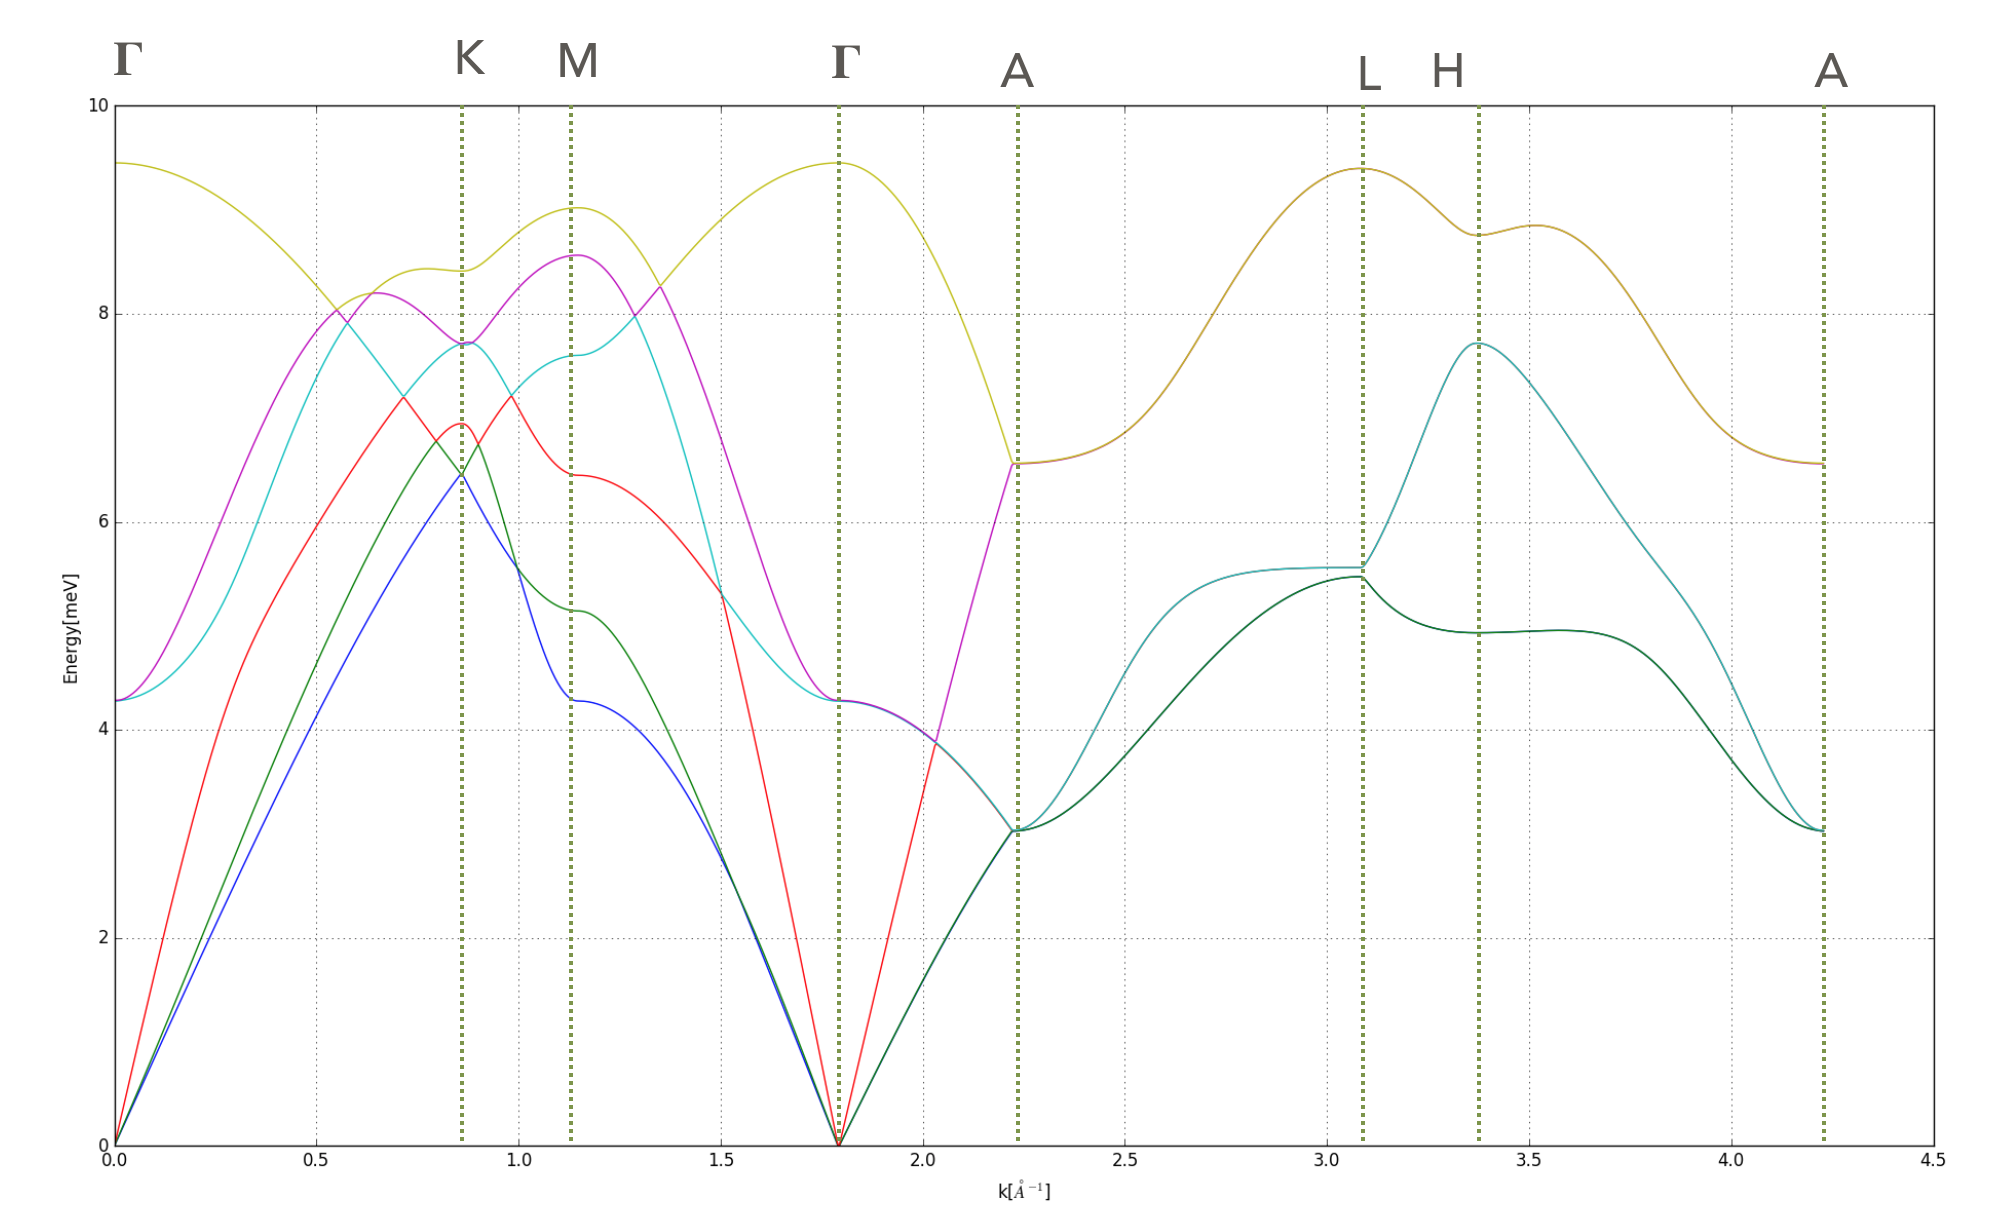
\includegraphics[width=12cm]{phonon_hcp.png}
        \caption{\it \label{phonon-hcp}Phon dispersion of HCP structure}
    \end{figure}

    \subsection{Spectrum of the FCC}

    In the case of the FCC configuration the cell contains only one atom and can be identified through the three vectors of coordinates\\
    \begin{minipage}{0.3\textwidth}
    \centering
    \begin{equation*}
    R_1 = a
    \begin{bmatrix}
        \frac{1}{\sqrt{2}} \\
        \frac{1}{\sqrt{2}} \\
        0 \\
        
    \end{bmatrix}
    \end{equation*}
    
    \end{minipage}
    \begin{minipage}{0.3\textwidth}
    \centering
    \begin{equation*}
    R_2 = a
    \begin{bmatrix}
        \frac{1}{\sqrt{2}} \\
        0 \\
        \frac{1}{\sqrt{2}} \\
    \end{bmatrix}
    \end{equation*}
    \end{minipage}
    \begin{minipage}{0.3\textwidth}
    \centering
    \begin{equation*}
    R_3 = a
    \begin{bmatrix}
        0 \\
        \frac{1}{\sqrt{2}}  \\
        \frac{1}{\sqrt{2}} \\
    \end{bmatrix}
    \end{equation*}
    \end{minipage}
    
    
    
    and that of the corresponding reciprocal lattice vectors can be constructed from those above and their coordinates are \\
    \begin{minipage}{0.3\textwidth}
        \centering
        \begin{equation*}
        G_1 = \frac{2\pi}{a}
        \begin{bmatrix}
            \frac{1}{\sqrt{2}} \\
            \frac{1}{\sqrt{2}} \\
            -\frac{1}{\sqrt{2}} \\
            
        \end{bmatrix}
        \end{equation*}
        
        \end{minipage}
        \begin{minipage}{0.3\textwidth}
        \centering
        \begin{equation*}
        G_2 = \frac{2\pi}{a}
        \begin{bmatrix}
            \frac{1}{\sqrt{2}} \\
            -\frac{1}{\sqrt{2}} \\
            \frac{1}{\sqrt{2}} \\
            
        \end{bmatrix}
        \end{equation*}
        \end{minipage}
        \begin{minipage}{0.3\textwidth}
        \centering
        \begin{equation*}
        G_3 = \frac{2\pi}{a}
        \begin{bmatrix}
            -\frac{1}{\sqrt{2}} \\
            \frac{1}{\sqrt{2}} \\
            \frac{1}{\sqrt{2}} \\
        
        \end{bmatrix}
        \end{equation*}
        \end{minipage}
    
        
        We can now define 
        \begin{equation}
            \Phi_{\alpha\beta}^{im}(r):=\frac{\partial^2 V(r)}{\partial r_{i,\alpha}\partial r_{m,\beta}}
        \end{equation}
        where the expression for the second derivative of the potential reads
        \begin{equation*}
            \frac{\partial^2 V(r)}{\partial r_{i,\alpha,g}\partial r_{m,\beta,f}} = \sum_j\left[\frac{\partial^2 v(r_{ij})}{\partial r_{ij}^2}\frac{(r_{ij})_{\alpha}(r_{ij})_{\beta}}{r_{ij}^2} + \frac{\partial v(r_{ij})}{\partial r_{ij}}\left(\frac{\delta_{\alpha\beta}}{r_ij}-\frac{(r_{ij})_{\alpha}(r_{ij})_{\beta}}{r_{ij}^3}\right)\right](\delta_{in}-\delta_{jn})
        \end{equation*}
        and from here the dynamical matrix
        \begin{equation}
            D_{\alpha\beta} = \frac{1}{M}\sum_j\left[\frac{\partial^2 v(r_{ij})}{\partial r_{ij}^2}\frac{(r_{ij})_{\alpha}(r_{ij})_{\beta}}{r_{ij}^2} + \frac{\partial v(r_{ij})}{\partial r_{ij}}\left(\frac{\delta_{\alpha\beta}}{r_ij}-\frac{(r_{ij})_{\alpha}(r_{ij})_{\beta}}{r_{ij}^3}\right)\right]\left(1-e^{i\underline{q}\underline{r}_{ij}}\right)
        \end{equation}
        The diagonalization of the former thus brings to the dispersion relation of the phonons. The calculated phonon dispersion is given in the figure \ref{phonon-fcc}
\begin{figure}[h]
    \centering
    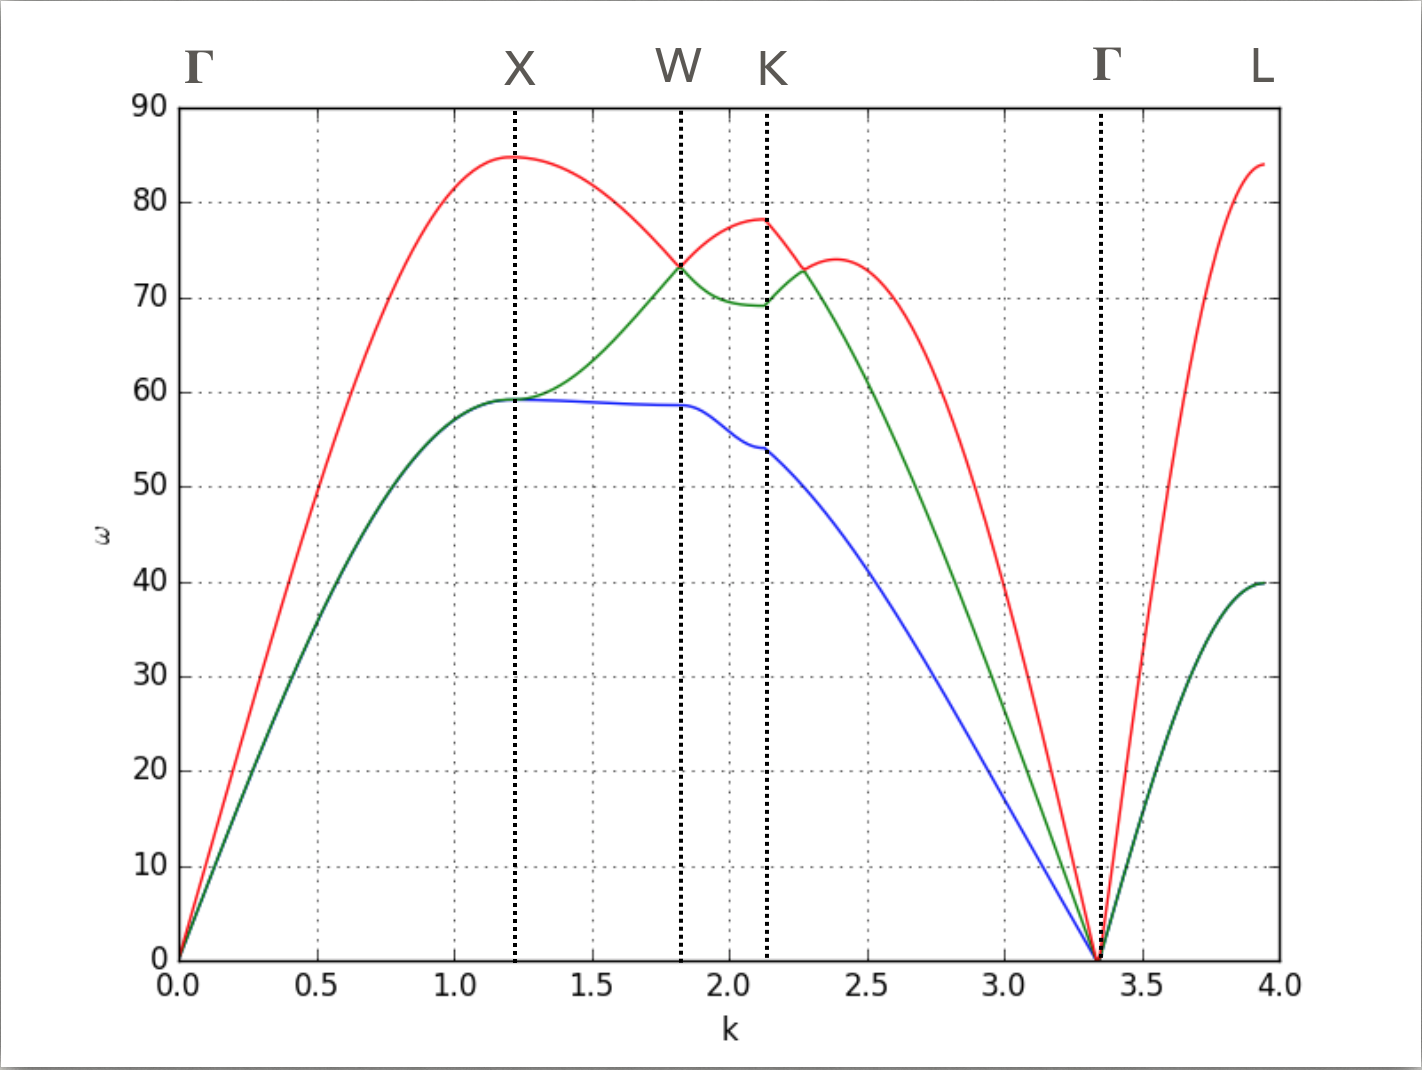
\includegraphics[width=12cm]{phonon_fcc.png}
    \caption{\it \label{phonon-fcc}Phon dispersion of FCC structure}
\end{figure}
%\bibliographystyle{alpha}
%\bibliography{sample}
\section{Calculation of Elastic Constants}

\end{document}